\documentclass[12pt,letterpaper]{article}
\usepackage[utf8]{inputenc}
\usepackage[spanish]{babel}
\usepackage{times}
\usepackage[left=3cm,top=2.5cm,bottom=2.5cm,right=2.5cm]{geometry}
\usepackage{graphicx}
\title{EV\_ 1\_ 3\_ circuitos\_ de\_ control\_ de\_ voltaje\_ y\_ corriente\_ con\_ tiristores.}


\begin{document}
\maketitle




\paragraph{ UNIVERSIDAD POLITÉCNICA DE LA ZONA METROPOLITANA DE GUADALAJARA}

\
\begin{figure}[h!]
\begin{center}


\includegraphics[scale=0.8]{Upzmg.png} 
\label{Upzmg}


\end{center}
\end{figure}


\

\author{Perez Alba Santiago Eduardo. \\ Romero Jauregui Osvaldo.
\

Fecha: 25 de Octubre del 2019.
\

Curso: Sep-Nov 2019.

\
Carrera: Ingeniería en Mecatronica.\

Docente: Moran Garabito Carlos Enrique}

\newpage

\section{Introducción:}

\
Durante la elaboración de esta practica se retomaran conocimiento previos y se utilizaran circuitos vistos anteriormente, como por ejemplo el de los relevadores y los optoacopladores, se retomaran conceptos de los mismos e incluirán nuevos como lo es el funcionamiento del Triac y el Diac. Durante su desarrollo se podrá ver el funcionamiento de cada uno de ellos para cumplir el objetivo de la practica.

\
\section{Objetivo:}

\
El objetivo principal de esta practica es observar la función que tendrán el TRIAC y el DIAC en conjunto con las resistencias, y relevadores para asi poder obtener distintas intensidades de luminosidad en el foco.

\section{Materiales:}
\begin{itemize}
\item Protoboard
\item 4n25 OptoAcopladores
\item Jumpers
\item Relevadores
\item TRIAC BT137
\item Resistencias Variadas
\item Fuentes DC
\item Clavija CA
\item Potenciometro
\end{itemize}

\section{Marco teórico:}

\
\textbf{TRIAC}: El TRIAC es un componente electrónico semiconductor de tres terminales para controlar la corriente. Su nombre viene del término \textbf{TRI}ode for \textbf{A}lternating \textbf{C}urrent = Triodo Para Corriente Alterna.

\
Un triac se utiliza para controlar una carga de CA(Corriente Alterna), semejante a como un transistor se puede utilizar para controlar una carga CC(Corriente Continua). En definitiva es un interruptor electrónico pero para corriente alterna. Los triac se utilizan en muchas ocasiones como alternativas de relé.
\

Su funcionamiento básico es cerrar un contacto entre dos terminales (anodo 1 y 2) para dejar pasar la corriente (corriente de salida) cuando se le aplica una pequeña corriente a otro terminal llamado "puerta" o Gate (corriente de activación).

\

\section{Desarrollo:}
\
Para iniciar la practica se tomó ventaja del circuito ya armado para la practica anterior la cual es el complemento de esta.
\

\begin{itemize}
\item Primero se analiza el circuito en conjunto con circuitos anteriores.
\item Después acoplaremos los componentes al circuito de manera que el foco y el TRIAC se añadieran en conjunto con las resistencias.
\end{itemize}
\

\begin{figure}[h!]
\begin{center}
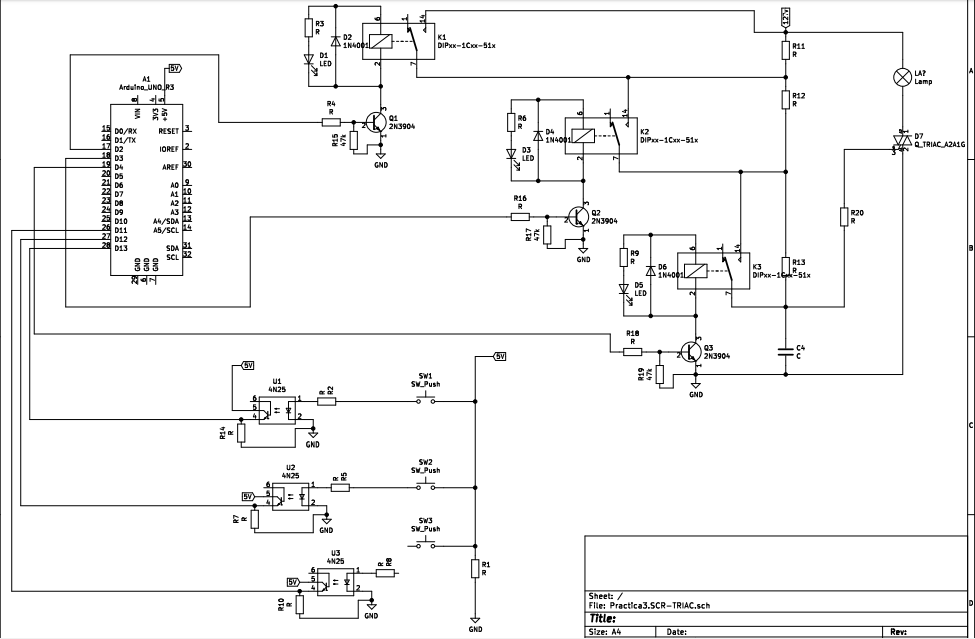
\includegraphics[scale=0.5]{Circuito.png} 
\caption{Esquema de Circuito-TRIAC}
\end{center}
\end{figure}

\newpage
Como era de esperarse, al momento de hacer las conexiones correctas el foco(CA) y las fuentes de DC nuestro componente prende con diferentes niveles de luminosidad al momento de que se da giro al potenciometro aumenta o bajara la luminosidad del mismo.
\

\begin{figure}[h!]
\begin{center}
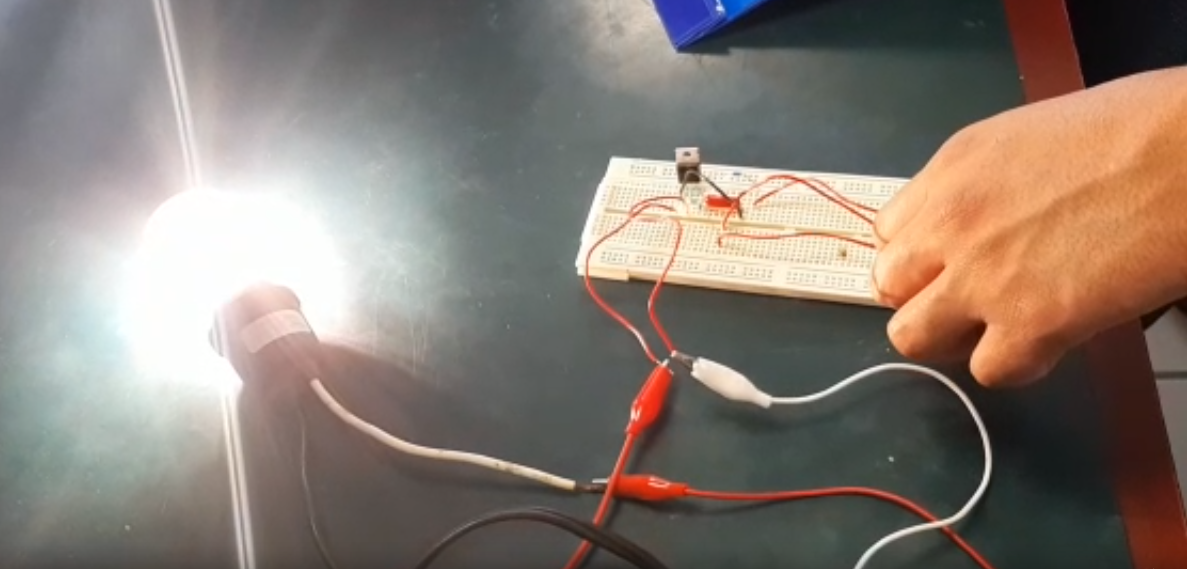
\includegraphics[scale=0.5]{Luminosidad-AltaR.png} 
\caption{Luminosidad máxima.}
\end{center}
\end{figure}

\
\begin{figure}[h!]
\begin{center}
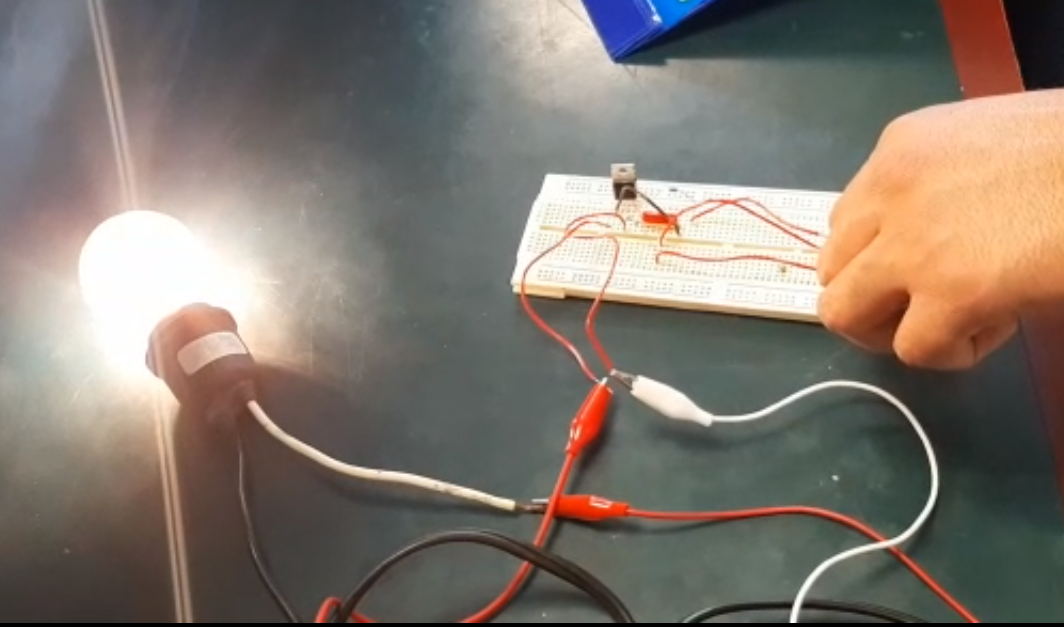
\includegraphics[scale=0.5]{Luminosidad-Media.png} 
\caption{Luminosidad Media.}
\end{center}
\end{figure}

\
\begin{figure}
\begin{center}
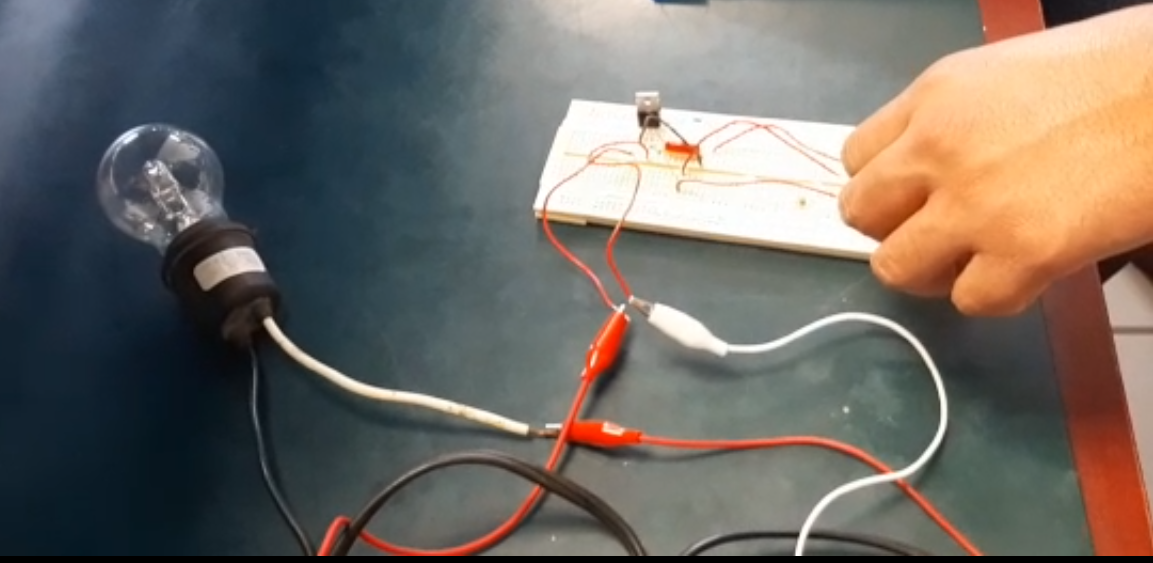
\includegraphics[scale=0.5]{Luminosidad-minima.png} 
\caption{Luminosidad mínima.}
\end{center}
\end{figure}

\
\section{Conclusiones:}
\
\begin{itemize}

\item Al momento en que se realizo la practica se encontraron ciertas dificultades para realizarlo como originalmente se muestra, ya que al momento de realizar la conexion de los relevadores con las resistencia y el TRIAC, no se lograba conseguir el cambio de luminosidad dentro del foco, por lo tanto se vio la necesidad de modificar el circuito original y se opto por adaptarlo a un potenciometro con el cual podríamos regular directamente la resistencia que tendría el circuito, mientras que la parte del TRIAC y el capacitor no se tuvo que hacer ninguna modificación, obteniendo los resultados de la [Figura 2].
\item En la practica se tuvo que buscar una alternativa ya que en el circuito original no se lograba conseguir el resultado esperado ya que había una diferencia entre las conexiones de relevador a las resistencia del TRIAC, por lo tanto se modifico el circuito y se adapto a un potenciometro y lograr regular la resistencia manualmente.
\end{itemize}
\end{document}